\chapter{Approximations}
\section{Global vs. local approximation}
\subsection{Global approximation}
	The first type of approximation consists in choosing a type of function (often polynomial) with parameters $a_i$ and defining $u_{approx}$ fitting the measurement points. Assume that we have the exact measurement $u_{exact,i}$ at 3 different point and that we want to approximate that by a second order polynomial: 
	
	\begin{equation}
	u_{exact}(x) \approx u_{approx}(x) = a_1 + a_2 x + a_3 x^2.
	\end{equation}
	
	By imposing this function to equal the exact values at the different points we get a system of three equations: 
	
	\begin{equation}
	\left\{
	\begin{aligned}
	&a_1 + a_2 x_1 + a_3 x^2_1 = u_{exact,1}\\
	&a_1 + a_2 x_2 + a_3 x^2_2 = u_{exact,2}\\
	&a_1 + a_2 x_3 + a_3 x^2_3 = u_{exact,3}
	\end{aligned}
		\right.
	\end{equation}
	
	As we have as many parameters as the number of measurement points, we have a single solution for the system. The approximation is often presented in the form:
	
	\begin{equation}
	u_{approx} (x)= [p_1(x) \ p_2(x) \dots] \left[\begin{array}{c}
	a_1\\
	a_2\\
	\vdots	
\end{array}	 \right] = \bm{p}(x)^T \bm{a}.
	\end{equation}
	
	where $\bm{p}(x)$ is a set of linearly independent functions, sometimes called the \textbf{basis} and $\bm{a}$ are the parameters of the approximation. Non linear expansion of parameters can also be encountered in a more advanced regression. The $a_i$ suffer from a lack of physical meaning, this is why we use the \textbf{nodal representation} where we explicitly use the measurement:
	
	\begin{equation}
	u_{approx} = u_{exact,1}N_1(x) + u_{exact,2}N_2(x) + \dots = \bm{N}(x)^T\bm{q}
	\end{equation}
	
	where $\bm{N}(x)$ contains the interpolation functions and $\bm{q}$ is the N exact nodal values. A widespread nodal approximation is the Lagrange interpolation, expressed assuming $x_i \neq x_j$: 
	
	\begin{equation}
	N_i (x) = \prod ^N _{j=1, j \neq i} \frac{x-x_j}{x_i-x_j}. 
	\label{eq:5.5}
	\end{equation}
	
	For example the first equation of the system will be in the case of three measurements: 
	
	\begin{equation}
	N_1(x) = \frac{(x-x_2)(x-x_3)}{(x_1-x_2)(x_1-x_3)}.
	\end{equation}
	
	The nodal approximations are defined to be interpolant ($u_{approx}(x_i) = u_{exact}(x_i)$), leading to:
	
	\begin{equation}
	N_i(x_j) = \delta _{ij}
	\end{equation}
	
	Schemes are global, since the parameter $a_i$ (or $u_i$) hold for the whole domain. This has a direct drawback when the number of samples increase. Indeed let's look to the figures below, at the beginning increasing the order of the polynomial allows a better fitting but then we get oscillations. This is known as \textbf{Runge's phenomenon}. 
	
	\begin{center}
	\begin{minipage}{0.55\textwidth}
	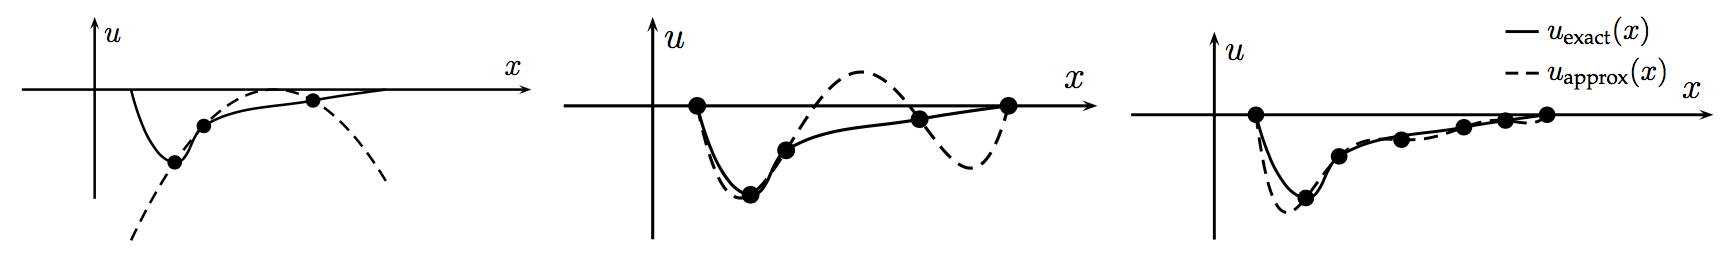
\includegraphics[scale=0.3]{ch5/1}
	\captionof{figure}{}
	\end{minipage}
	\begin{minipage}{0.4\textwidth}
	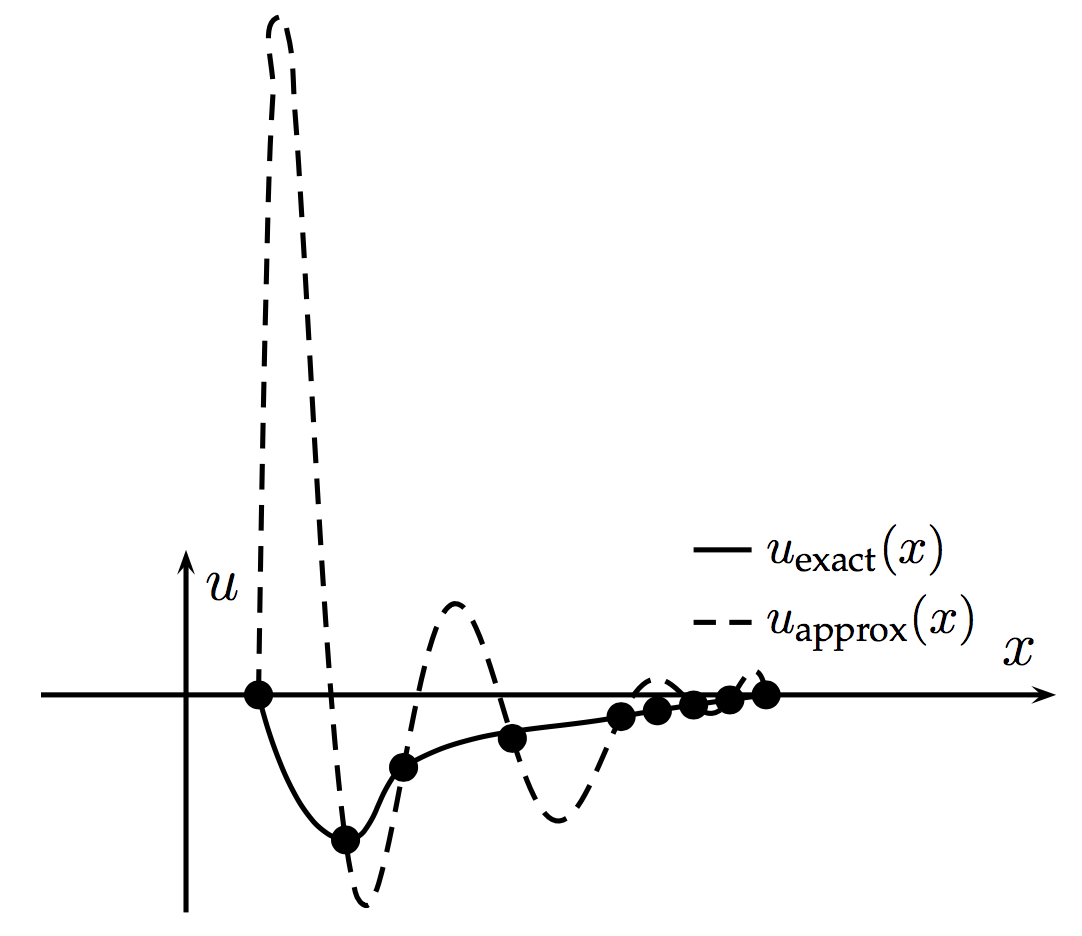
\includegraphics[scale=0.3]{ch5/2}
	\captionof{figure}{}
	\end{minipage}
	\end{center}
	
	The problem can be mitigated by using a \textbf{least square approach}. Instead of a pure interpolation that forces to pass exactly on the samples, we will use an \textbf{ordinary least square} model where the order of the polynomial m will be independent of the number of sample points N ($m\leq N$). The parameters are obtained by minimization of the error $e_{LS}$ between the approx and the exact function: 
	
	\begin{equation}
	\bm{a} = \arg \min _a \left\{ e_{LS} \equiv \frac{1}{2}\sum _{i=1}^N \left(u_{exact,i}-\bm{p}(x_i)^T\bm{a}\right)^2 \right\} = \left( \bm{P}^T\bm{P} \right)^{-1} \bm{P}^T \bm{q};
	\end{equation}
	
	where $\bm{P}$ contains the basis evaluated at the sample points $x_i$: 
	
	\begin{equation}
	\bm{P} = \left[  
	\begin{array}{cccc}
	p_1(x_1) & p_2(x_1) & \dots & p_{m+1}(x_1)\\
	\vdots & & & \vdots \\
	p_1(x_N) & p_2(x_N) & \dots & p_{m+1}(x_N)
	\end{array}
	\right]
	\end{equation}
	
	To give a higher influence on the samples located close to the point x where the prediction is required, an additional weight function can be used to obtain a higher impact on the nodes $x_i$ close to $x$. This $w_i = w(x;x_i)$ is usually a function decreasing monotonically with the distance $||x-x_i||$. This makes the minimum depends on x: 
	
	\begin{equation}
	\begin{aligned}
	\bm{a}(x) &= \arg \min _a \left\{ e_{LS} \equiv \frac{1}{2}\sum _{i=1}^N w_i \left(u_{exact,i}-\bm{p}(x_i)^T\bm{a}\right)^2 \right\} = \left( \bm{P}^T\bm{W}\bm{P} \right)^{-1} (\bm{P}^T\bm{W}) \bm{q};\\
	\bm{W} &=
	\left[
	\begin{array}{ccc}
	w_1\equiv w(||x-x_1||) & 0 & \dots\\
	0 & w_2\equiv w(||x-x_2||) & \dots\\
	\vdots & & \vdots
	\end{array}
	\right]
	\end{aligned}
	\end{equation}
	
	If the approximation is non zero in a only in a vicinity around the guess point x, and vanishes everywhere else, the technique is called \textbf{moving least square}. 
	
\subsection{Local approximation}
	Here we divide from the beginning a local approximation through \textbf{nodal approximation by sub-domain}:
	
	\begin{itemize}
	\item[•] domain $V$ is divided into sub-domains $V^e$;
	\item[•] an approx is build for each $V^e$, the parameter can depend on the other sub-domains parameters (splines in CAD);
	\item[•] the nodal approx on each $V^e$ only envolves the variables attached to the nodes within $V^e$ and its boundary;
	\item[•] functions $u^e(x)$ are continuous within $V^e$ and respect continuity conditions across sub-domains;\\
	
	\item[•] $V^e$ are the \textbf{finite elements}
	\item[•] the points where the approximations are forced to coincide with the exact value are the \textbf{interpolation nodes}; the coordinates of those points are the \textbf{nodal coordinates};
	\item[•] the values $u_i = u_{approx}(x_i) \equiv u_{exact}(x_i)$ are the nodal variables.  
	\end{itemize}
	
	\begin{center}
	\begin{minipage}{0.45\textwidth}
	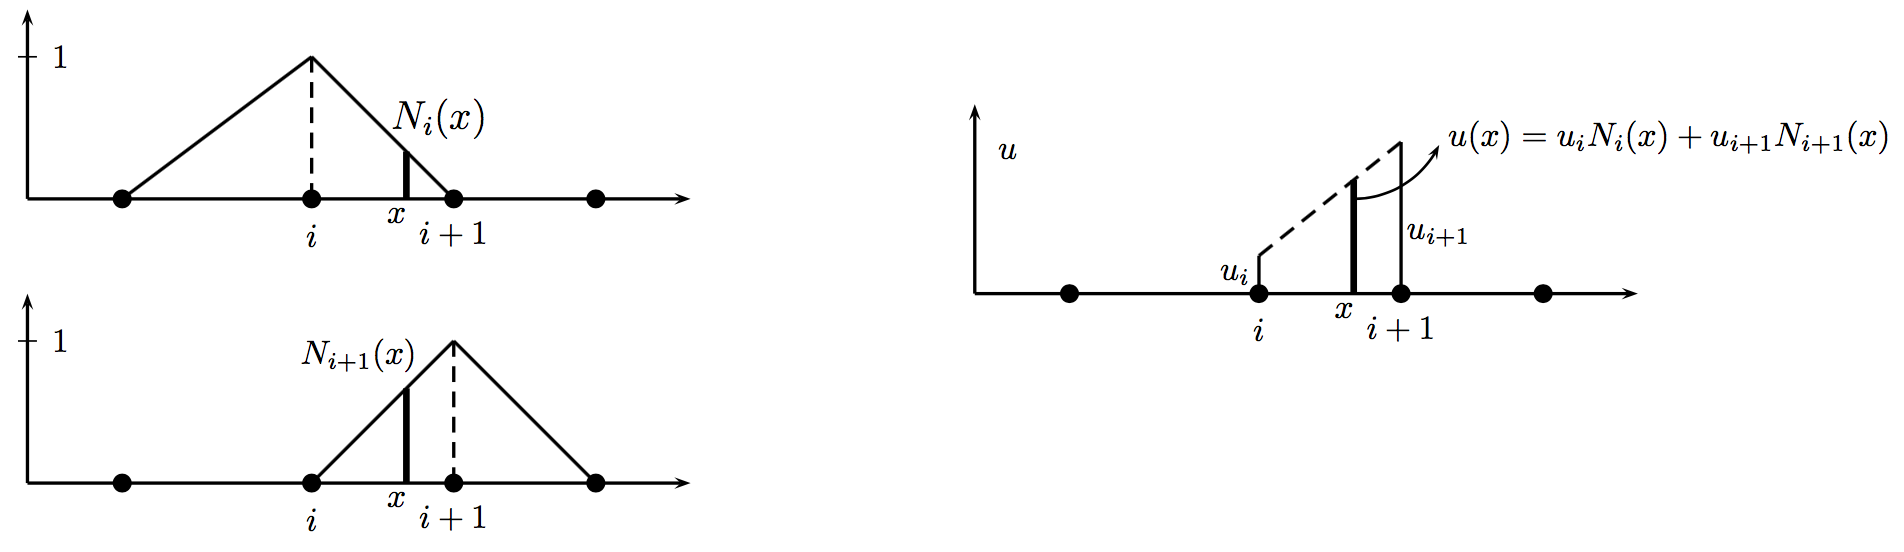
\includegraphics[scale=0.22]{ch5/3}
	\captionof{figure}{}
	\label{fig:5.3}
	\end{minipage}
	\begin{minipage}{0.45\textwidth}
	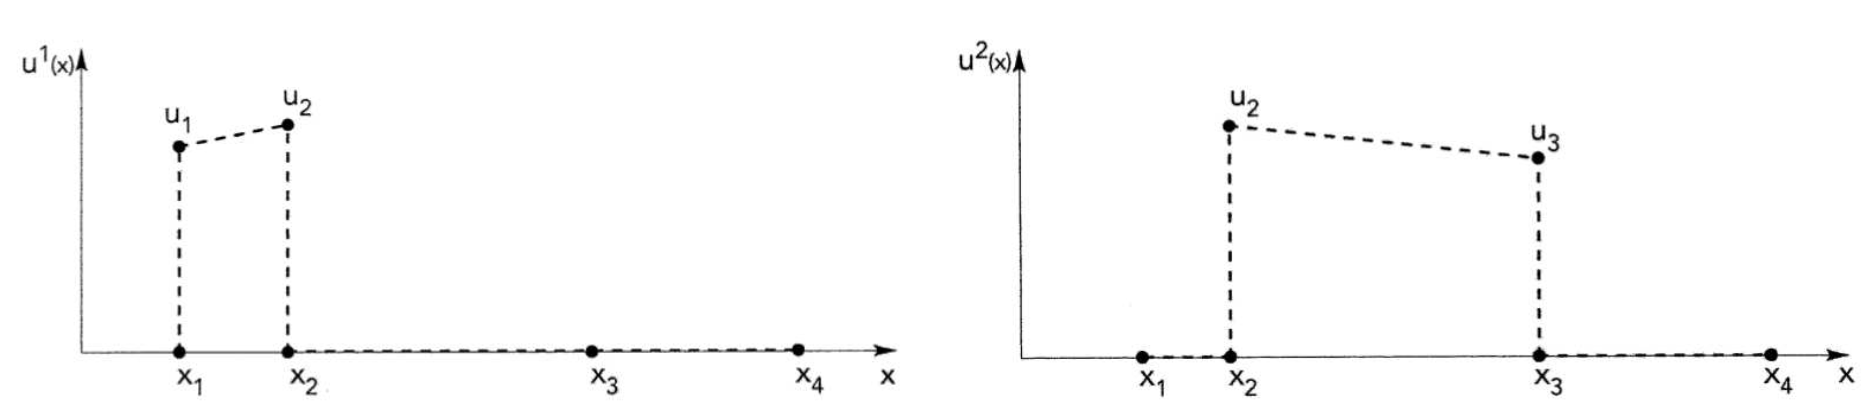
\includegraphics[scale=0.22]{ch5/4}
	\captionof{figure}{}
	\label{fig:5.4}
	\end{minipage}
	\end{center}
	
	The simplest approximation consists in a piecewise first-order interpolation. On the above figures we can see an illustration in a one-dimensional problem with four nodes, on $V^1$ only the first two  nodes are taking place in the approx:
	
	\begin{equation}
	u_{approx}^{V^1} = N_1(x) u_1 + N_2 u_2,
	\end{equation}
	
	with the definition \eqref{eq:5.5} and same for $u_{approx}^{V^2}$ and $u_{approx}^{V^3}$. $N_i$ are also called \textbf{shape functions}. This is illustrated on \autoref{fig:5.3}. We see that the shape function is associated to a given node $x_i$ and is different from zero on the elements containing it. This principle can be generalized in 3D (\autoref{fig:5.6}). 
	
	\begin{center}
	\begin{minipage}{0.5\textwidth}
	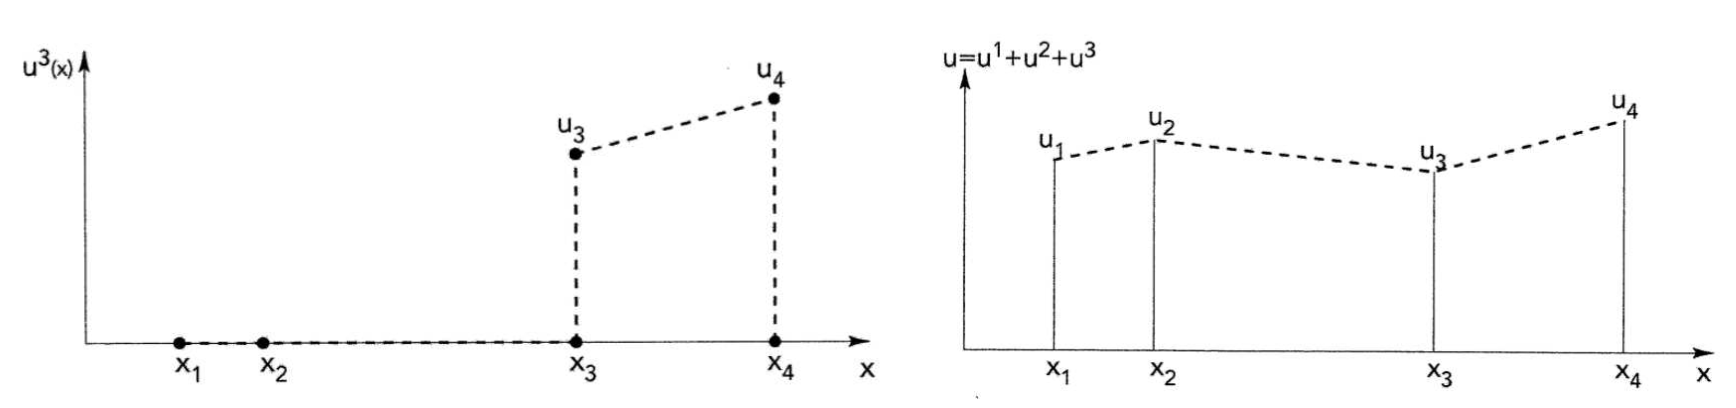
\includegraphics[scale=0.3]{ch5/5}
	\captionof{figure}{}
	\label{fig:5.5}
	\end{minipage}
	\begin{minipage}{0.45\textwidth}
	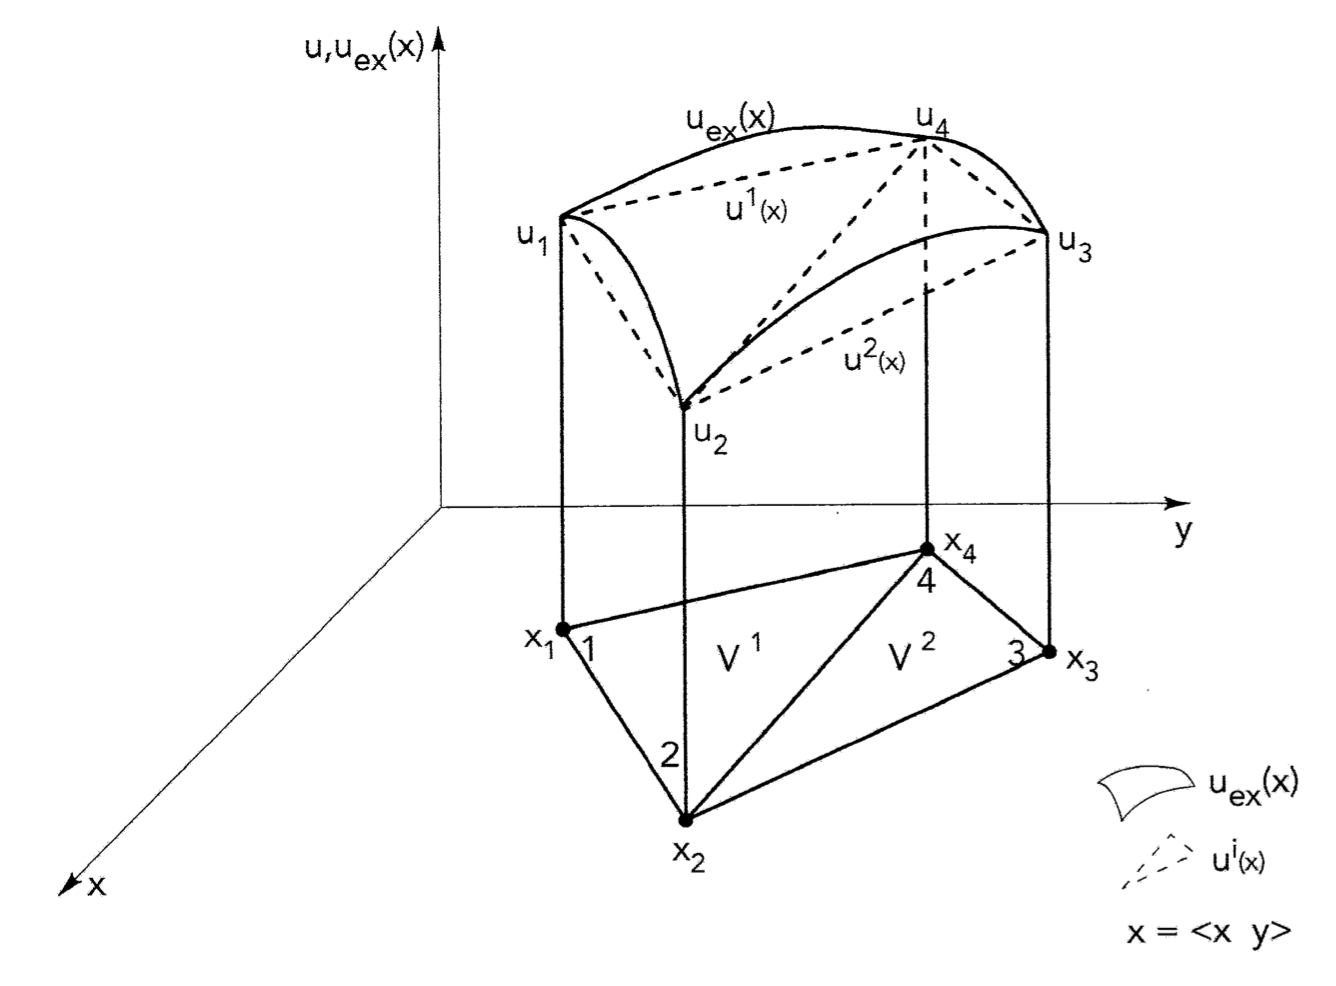
\includegraphics[scale=0.26]{ch5/6}
	\captionof{figure}{}
	\label{fig:5.6}
	\end{minipage}
	\end{center}
	
	The finite eement approximation offers 4 advantages:
	
	\begin{itemize}
	\item[•] local behavior, one node influence only its neighborhood;
	\item[•] low order polynomial in order to avoid the Runge's effect;
	\item[•] interpolation at the nodes;
	\item[•] physical interpretation of the coefficients.
	\end{itemize}
	
	Moreover as the shape function is non zero only for the $x_i$ belonging to the element $e$, we can write for the whole discretized domain:
	
	\begin{equation}
	u_{approx} = N^e(x) q^e = N(x) q
	\end{equation}
	
	where $q^e$ contains the nodal values of $u$ on the element, whereas $q$ nodal values for the whole domain. 